\section{Introduction}
\subsection{Why we want qunantum computer}
Computers are undoubtedly one of the most useful, powerful, and essential tools in the twenty-first century. We can use them to view the latest news in the world, train models on auto-driving cars, and do ab initio calculations for diverse material. Although Gordon Moore correctly predicted that the processors would double the number of transistors per year in the past 60 years, electron tunneling and heat generation due to the growing density of transistors are challenging the known Moore's law.

The Quantum computer is considered a powerful supplement to the classical computer in simulating nature due to its overwhelming advantage in inherent parallel computing capability. Unlike classical bits 0 and 1, quantum bits, namely qubit, can form a superposition of $|0\rangle$ and $|1\rangle$ with phase. This property gives quantum computers extraordinary power to solve challenging questions such as the decomposition of sizeable prime number\cite{RN74}. Due to the powerful quantum parallelism, people also study the quantum algorithm of ray tracing in rendering images for games\cite{RN76}.

The community now positions superconducting qubits as a platform for noisy intermediate scale quantum (NISQ) computing that performs calculations outside of classical algorithms but with limited logical error-corrected qubits\cite{RN1}. Nevertheless, quantum computers can still outperform classical computers in specific calculations. Some people call this surpass 'quantum supremacy'\cite{RN44}, or more gently 'quantum advantage'\cite{RN77}. Scientists and engineers are trying to push the performance of quantum computing forward through, for example, mitigating noise and gate set improvement to the scalable fault-tolerant quantum computer. Until then, we can implement some more heavily-loaded industrial computational tasks and safely say we have reached the quantum computer era.

There are several ways to realize quantum computers. Superconducting qubit is one of the most promising competitors owing to their scalability, fast gate time, and relatively mature fabrication technique. Despite their disadvantages in fast decoherence and the need for a cryogenic environment, superconducting qubits still prosper around the quantum computing community and develop swiftly. A recent paper utilizes a 62-qubit programmable superconducting processor to perform quantum algorithm\cite{RN43}. Among all the types of superconducting qubits, transmon, namely transmission-line shunted plasma oscillation qubits, is a popular type of charge-insensitive qubit investigated by many labs and companies such as IBM. Based on the idea of transmon, to tune the frequency of the qubit to explore the optimal working regime, people will use superconducting quantum interference device (SQUID) to introduce flux, therefore phase change on the junction. We, in this thesis, use gate-tunable S-Sm-S nanowires to act as the Josephson junction. By defining the gate beneath the junction, we can tune the Fermi energy of the junction, thus the qubits' frequency. In this thesis, we propose a path of using tantalum-coated with shadow in-situ growth S-Sm-S junction InAs nanowire as Josephson junction in gatemon and tantalum as capacitors and control lines as superconducting qubits. We do both DC transport measurements on the tantalum nanowires to prove the possibility of utilizing them as Josephson junction and high-frequency measurement on resonator to show the high quality factor of tantalum.  

\subsection{Basic quantum computing}
\subsubsection{Classical bit to qubit}
Classically, we use binary representation, 0 and 1, in modern transistor computers and can implement elementary arithmetic by utilizing different gates' combinations. It's worth emphasizing here that each bit is definite, such as 5V in the circuit stands for one and 0V stands for zero. No intermediate bit is allowed like 3V stands for 0.6. Meanwhile, the gate operations like adder can change the number of bits, leading to loss of information during calculations.

When we move to the quantum world, things are very different. Think of a single electron. We learn from Stern–Gerlach experiment that the angular momentum on the z direction can be quantized, and we name it spin with spin up $|\uparrow\rangle$ and down $|\downarrow\rangle$, which represents $|0\rangle$ and $|1\rangle$. However, prior to the measurement, the spin's output can't be written as any function with fixed variables, but only the probabilistic function. It means that quantum mechanics is not local and against the hidden-variable theory. This is the well-known Bell's theorem\cite{RN52} and has been experimentally proved\cite{RN53}. The only way to represent such a state is to use complex number $\alpha$ and $\beta$ like $|\psi\rangle = \alpha|0\rangle + \beta|1\rangle$ with normalization condition $|\alpha|^2 + |\beta|^2 = 1$. The superposition state $|\psi\rangle$ here, in quantum information, can be called a qubit.

An arbitrary pure state spin's, generally two-level systems, density matrix can be described as:
\begin{equation}\label{densitymatrix}
    \rho = |\mathbf{\psi}\rangle\langle\mathbf{\psi}| = \frac{1}{2} (\mathbf{I} + \mathbf{s\cdot\sigma})
\end{equation}
with Bloch vector $\mathbf{s} = (x, y, z)$ and Pauli matrix $\sigma$. For convenience, we use a Bloch sphere to represent the qubit (fig). Let $\mathbf{s} = ( \sin{\theta}\cos{\phi}, \sin{\theta}\sin{\phi}, \cos{\theta})$ we now gain a qubit with the wave function: 
\begin{equation}
    |\psi\rangle = cos\frac{\theta}{2}|0\rangle + e^{i\phi}\sin{\frac{\theta}{2}}|1\rangle
\end{equation}
The coordinate $(\theta, \phi)$ indicates a pure state point on the surface of the Bloch sphere. If a mixed state, that is $\text{Tr}(\rho^2) \neq 1$, the vector points inside the sphere. For example, the process of qubit decoherence corresponds to a trace from the sphere surface to the inner part.
\begin{figure}[h!]
    \centering
    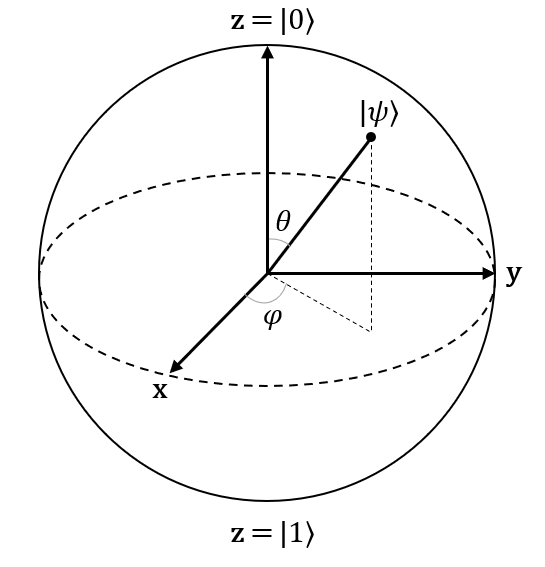
\includegraphics[width=0.4\textwidth]{Pic/Blochsphere.png}
    \caption{The illustration of Bloch sphere. Every point on the surface of the sphere stands for a pure state (for example, the point on the north pole at the end of the z-axis can be $|0\rangle$).}
    \label{fig:my_label}
\end{figure}
Multi qubits entanglement is another important characteristic different from classical computing. The entanglement as a non-local correlation mathematically means that the many qubits' states can't be written as the direct product of single qubit's state. A two qubits, A and B, system can have a maximally entangled basis, Bell basis:
\begin{equation}
    \begin{array}{cc}
         |\Phi^+\rangle =& \frac{1}{\sqrt{2}}(|0\rangle_A\otimes|0\rangle_B + |1\rangle_A\otimes|1\rangle_B)  \\
         |\Phi^-\rangle =& \frac{1}{\sqrt{2}}(|0\rangle_A\otimes|0\rangle_B - |1\rangle_A\otimes|1\rangle_B)  \\
         |\Psi^+\rangle =& \frac{1}{\sqrt{2}}(|0\rangle_A\otimes|1\rangle_B + |1\rangle_A\otimes|0\rangle_B)  \\
         |\Psi^-\rangle =& \frac{1}{\sqrt{2}}(|0\rangle_A\otimes|1\rangle_B - |1\rangle_A\otimes|0\rangle_B) 
    \end{array}
\end{equation}
Take $ |\Phi^+\rangle$ as an example. If qubit A collapses to the ground state, we can definitely say that qubit B is also in the ground state theoretically, and vice versa. Therefore the $ |\Phi^+\rangle$ state can't be written as any form of $|A\rangle \otimes|B\rangle$. 

Superposition and entanglement are the foundation of the quantum technology field, including quantum communication, quantum simulation, and quantum computing, and the reason for fast parallel computation in quantum computers. We can initialise a quantum state $\psi = \sum_{k=1,2..N}p_k|s_0s_1...s_N\rangle$, with $s_k$ the state of qubit k, and compute $2^N$ state simultaneously in a single step. This property endows exponential acceleration in certain calculations, like Shor's algorithm for integer prime factorization.

\subsubsection{Quantum logic gate}
Classically, the logic gates include non-reversible operation AND, OR with 2 bits in then 1 bit out. Unlike the classical situation, quantum gates are represented as unitary operators, meaning no information is lost during the calculation. Any single qubit gate operation can be represented as pivot rotation of vector on Bloch sphere:
\begin{equation}
    \mathbf{R}(\mathbf{n}, \varphi) = \exp(-i\frac{\varphi}{2}\mathbf{n}\cdot{\sigma}) = \cos{(\frac{\varphi}{2}})\cdot I - i\sin{(\frac{\varphi}{2})}\mathbf{n}\cdot\sigma
\end{equation}
where $\mathbf{n} = (\sin{\theta}\sin{\phi}, \sin{\theta}\cos{\phi}, \cos{\theta})$ and $\varphi$ the rotation angle. For example, we can construct a Hadamard gate:
\begin{equation}
    H = \frac{\sqrt{2}}{2}
    \begin{pmatrix}
1 & 1 \\
1 & -1 
\end{pmatrix}
\end{equation}
This gate operation will bring state $|0\rangle$ to $|+\rangle = \frac{1}{\sqrt{2}}(|0\rangle+|1\rangle)$. 

To realize entanglement between two qubits, we also need two qubits gate, like Control-NOT (CNOT) gate under $|00\rangle, |01\rangle, |10\rangle, |11\rangle$ basis:
\begin{equation}
    CNOT = 
    \begin{pmatrix}
1 & 0 & 0 & 0 \\
0 & 1 & 0 & 0 \\
0 & 0 & 0 & 1 \\
0 & 0 & 1 & 0 
\end{pmatrix}
\end{equation}
. This gate maps $|10\rangle$ to $|11\rangle$, and  $|11\rangle$ to  $|10\rangle$. As shown in Fig.\ref{phi+state}, with the combination of Hadamard gates and CNOT gates, we can prepare a $|\Phi^+\rangle$ state.
\begin{figure}[h!]
    \centering
    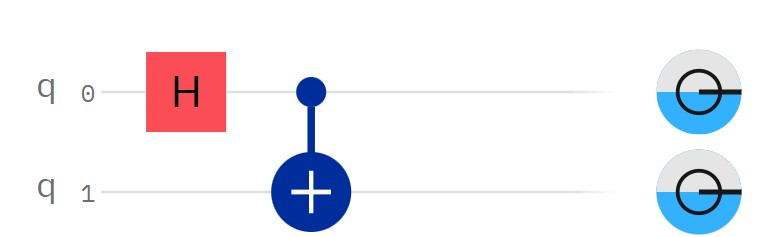
\includegraphics[width=0.5\textwidth]{Pic/Phi+state.jpg}
    \caption{The two qubits both start with initial state $|0\rangle$. In the first operation, qubit 0 undergoes a Hadamard gate, and the qubit state becomes $\frac{1}{\sqrt{2}}(|0\rangle+|1\rangle)\otimes|0\rangle$. After the CNOT gate, the state becomes $\frac{1}{\sqrt{2}}(|0\rangle\otimes|0\rangle + |1\rangle\otimes|1\rangle)$, the $|\Phi^+\rangle $state.}
    \label{phi+state}
\end{figure}

\subsubsection{Quantum measurement}
In quantum mechanics, measurement operation equals to the average of a certain operator of some wave function:
\begin{equation}
    \langle\mathbf{F}\rangle = \langle\psi|\mathbf{F}|\psi\rangle
\end{equation}
In qubit, we perform projection measurement, a single shot readout with operator $\mathbf{P}_s = |s\rangle\langle s|$, s is 0 or 1. After thousand times of measurement, the probability of qubit in $|s\rangle$ state, $|\alpha|^2$ or $|\beta|^2$, is obtained. Quantum non-demolition (QND) measurement is another important concept. With QND, the qubit system remains in the computational subspace and can be repeatedly measured. For example, if we find the qubit is in $|1\rangle$ state, this $|1\rangle$ state can be used as a new initial state for future operations. Dispersive readout, a common QND measurement method for qubits, is performed with far detuning between the resonator and qubit. When the coupling rate of the resonator and qubit $g$, and the resonator linewidth $\kappa$ is much lower than the frequency detuning $\Delta \rr g, \kappa$, the readout system is in the dispersive limit and without direct energy exchange to the qubit.

Projection measurement doesn't provide enough information for the density matrix of the whole qubit system. We need to introduce quantum state tomography to get all the elements in the density matrix. In the case of a single qubit, from Eq.\ref{densitymatrix} we can see that if we measure $\sigma_x, \sigma_y, \sigma_z$, we can obtain $(x,y,z)$ and then the density matrix. In a multi-qubits system, we can use a neural network to get the density matrix swiftly\cite{RN55}.

\subsubsection{Decoherence}
The word noise in NISQ indicates decoherence in qubits. The qubit system is unavoidably connected to the environment because we need to read out the information inside the system. Therefore the qubit and environment undergo energy exchange and phase variation. We often consider this event a stochastic process.
We usually sort it into two kinds of relaxation. One is energy relaxation, or longitudinal relaxation\cite{RN8}. In the Bloch sphere, the trace of it indicates a straight line from $|1\rangle$ to $|0\rangle$ through the sphere center. The average time for the evolution is usually written as $T_1$. We can use the Kraus operator to describe the process quantitatively\cite{RN34}:
\begin{equation}
    \rho(t+\Delta t) = \sum_{i=0,1} K_i \cdot \rho (t) \cdot K_i^\dagger
\end{equation}
where:
\begin{equation}
    K_0 = \begin{pmatrix}
1 & 0 \\
0 & e^{-\Delta t/2T_1}
\end{pmatrix},
K_1 = \begin{pmatrix}
0 & \sqrt{1-e^{-\Delta t/T_1}} \\
0 & 0
\end{pmatrix}
\end{equation}
After evolving $\Delta t$ time, the density matrix becomes:
\begin{equation}
    \rho(t+\Delta t) = \begin{pmatrix}
\rho_{00}(t) + (1-e^{-\Delta t / T_1)}\rho_{11}(t) & \rho_{01}(t)e^{-\Delta t/2T_1} \\
\rho_{10}(t)e^{-\Delta t/2T_1} & \rho_{11}(t)e^{-\Delta t/2T_1}
\end{pmatrix}
\end{equation}
The other relaxation is called dephasing, also pure dephasing time $T_2^\ast$. The trace of it is a straight line from a point on the equator on the Bloch sphere to the center. The three Kraus operators to describe the system are:
\begin{equation}
    K_0 = e^{\Delta t/2T_2^\ast}, 
    K_1 = \begin{pmatrix}
\sqrt{1 - e^{{\Delta t/T_2^\ast}}} & 0 \\
0 & 0
\end{pmatrix},
K_2 = \begin{pmatrix}
0 & 0 \\
0 & \sqrt{1 - e^{\Delta t/T_2^\ast}}
\end{pmatrix}
\end{equation}
, and the density matrix becomes:
\begin{equation}
    \rho(t+\Delta t) = \begin{pmatrix}
\rho_{00}(t)& \rho_{01}(t)e^{-\Delta t/T_2^\ast} \\
\rho_{10}(t)e^{-\Delta t/T_2^\ast}
& \rho_{11}(t)
\end{pmatrix}.
\end{equation}
Pure dephasing only affects the off-diagonal terms in the density matrix. We shall notice that the energy relaxation also affects the off-diagonal terms, so we define a dephasing or transverse relaxation time $T_2$:
\begin{equation}
    \frac{1}{T_2} = \frac{1}{2T_1} + \frac{1}{T_2^\ast}
\end{equation}

\subsubsection{Quantum information}
In classical information, we have Shannon entropy $\text{H} = -\sum_{i=1}^n P(x_i)\log P(x_i)$. The quantum analog version is Von Neumann entropy: \begin{equation}
    S(\rho) = -\text{Tr}(\rho\ln\rho).
\end{equation}
This entropy measures the uncertainty of a quantum system and can be potentially used in quantum machine learning\cite{RN57}. 

There are several important theorems in quantum information\cite{RN34}:
\begin{description}
    \item[no-cloning theorem] Any ket state $|\Psi\rangle$ cannot get a duplication.
    \item[no-converting theorem] No quantum state can be transferred into classical bits.
    \item[no-deleting theorem] The number of qubits after gate operations are conserved, and no destructive gate exists in the quantum world.
    \item[no-broadcast theorem] Prevent an arbitrary qubit from delivering to multiple recipients. 
    \item[no-hiding theorem] The information in the qubit never disappears. It may leak into the subspace of the environment but not vanish.
\end{description}
Notice that although there are five theorems, some of them can be mutually agreed upon. For example, from the no-cloning theorem, we can confidently say a no-broadcast theorem because if the latter is wrong, there will be more than one duplication of the qubit, which doesn't make sense. The no-converting theorem is called the no-transportation theorem in some textbooks. Still, since we can actually do quantum teleportation, it is more reasonable to use this name of the theorem instead.

\subsubsection{Physical realization of quantum computer}
The ultimate question after the theory is if we can realize quantum computers in the physical world. Physicist D.DiVincenzo raised five criteria on quantum computing.\cite{RN59}
\begin{description}
    \item 1. The system is scalable and along with well-controlled qubits
    \item 2. Qubits can be initialized to a simple state.
    \item 3. Much longer coherence time compared to single qubit gate manipulation time.
    \item 4. A universal gate set.
    \item 5. Decent qubit readout system.
\end{description}
Scientists have used many physical systems to build controllable quantum bits, some of which partly satisfy DiVincenzo's criteria.

Other than quantum computing, quantum technology applications also include quantum key distribution (QKD). In 2017, a Chinese team \cite{RN58} successfully demonstrated QKD over a distance of 1200 kilometers.

\subsection{Layout of the thesis}
In \textbf{Chapter 2}, we investigate the basic concept of quantum computing, including quantum information and two-level systems. Additionally, we introduce the physics of charge qubit, transmon, and gatemon, then circuit quantum electrodynamics (circuit QED) and its implementation in superconducting qubit systems. \textbf{Chapter 3} describes the simulation and fabrication of our devices. Then the setup on both DC transportation measurement on lock-in and high-frequency measurement on VNA. \textbf{Chapter 4} involves three DC measurement data of shadow S-Sm-S junction tantalum InAs nanowires in both board station (with $T_{env} \approx 5 K$) and in dilution fridge (with $T_{env} \approx 25 mK$). \textbf{Chapter 5} shows the high-frequency transmission measurement of wet etched sputter tantalum resonator, with different cleaning processes and shielding techniques, in our dilution fridge.